\begin{cadre}
Souvent, les situations que l'on veut étudier en physique sont complexes. Imaginons un skieur qui descend une piste : ses deux skis glissent sur la neige, le poids de son corps est réparti inégalement sur les deux skis, l'air le freine, la piste n'est pas parfaitement lisse, etc. Si l'on veut pouvoir étudier le mouvement du skieur (notre \emph{objet} d'étude), il faut être capable de simplifier au maximum la situation, mais pas trop ! Il faut donc \emph{négliger} tout ce qu'il n'est pas utile de prendre en compte. Par exemple on peut négliger le frottement des skis sur la neige en faisant la supposition que la glisse est parfaite et que les frottements de l'air sont bien plus forts que les frottements ski--neige. De même, le skieur et son matériel pourront être assimilé à un point unique dont la masse est celle du skieur et de son équipement. Le poids du skieur, qui est réparti sur l'ensemble de la surface des skis, pourra alors être supposé appliqué uniquement sur ce point, etc. C'est ce qu'on appelle \emph{modéliser} la situation : il faut parvenir à la situation la plus simple possible qui corresponde encore suffisamment à la réalité.  

\vspace{.5em}

Voilà le rôle du physicien : à partir d'un objet dans une situation complexe, il doit trouver une modélisation qui corresponde suffisamment à la réalité pour pouvoir prévoir l'évolution du mouvement de l'objet étudié. Au fil des deux premiers chapitres, nous allons apprendre à modéliser une situation physique pour pouvoir l'étudier et prédire comment va varier son mouvement. Ce premier chapitre s'attelle à la modélisation de l'action mécanique.

\vspace{.5em}

Dans un second temps il sera question de la modélisation d'une situation physique à l'aide d'un diagramme objets-interactions qui, comme son nom l'indique, regroupe sur un même diagramme tous les objets en présence et toutes les interactions entre ces objets et un objet particulier : le système étudié. Ce sera également l'occasion de dresser une liste des différentes forces (interactions) que nous allons rencontrer cette année.
\end{cadre}

\section{Introduction}

Ce premier chapitre, où il est question de forces et d'interactions, fait partie de la \emph{mécanique}. 

\textsl{La mécanique (du grec ancien « l'art de construire une machine ») est une branche de la physique dont l'objet est l'étude du mouvement, des déformations ou des états d'équilibre des systèmes physiques. Cette science vise ainsi à décrire les mouvements de différentes sortes de corps, depuis les particules subatomiques avec la mécanique quantique, jusqu'aux galaxies avec la mécanique céleste.}\hfill{\footnotesize(Définition de Wikipedia)}

\section{L'objet étudié : le système}

Lorsqu'on étudie une situation physique dans laquelle plusieurs objets sont présents, on doit distinguer un objet en particulier qui nous intéresse. C'est cet objet que l'on étudie : on veut connaître sa position, sa vitesse, comment va évoluer son mouvement, etc. L'objet qu'on étudie est appelé le \textbf{\MotDefinition{système}{}}. Pour le distinguer, on le note entre accolades, par exemple : \{skieur\}.


\section{Modélisation de l'objet étudié}

Les objets que l'on étudie sont modélisés par un unique point, dont la masse est celui de l'objet. Ce point n'est pas choisi au hasard : c'est le centre de gravité de l'objet.

\begin{center}
    \includegraphics[width=.5\linewidth]{cdg}
\end{center}



\section{Action mécanique}

Lorsqu'un objet agit sur un autre objet, on parle d'\textbf{\MotDefinition{action mécanique}{}}.

Si les deux objets se touchent, on dit qu'il y a \textbf{action mécanique de contact} (exemple : un homme qui pousse une armoire). Par contre, si les deux objets ne se touchent pas, on dit qu'il y a \textbf{action mécanique à distance} (ex : un aimant qui attire un morceau de fer).   

\begin{aconnaitre}[Action mécanique]
Une \textbf{action mécanique}, exercée par un objet (l'acteur) sur un autre objet (le receveur, ici le système), peut :
\begin{itemize}
\item mettre en mouvement le système ;
\item modifier la trajectoire du système ;
\item déformer le système.
\end{itemize}

\vspace{.5em}

Plus la masse du système est faible, plus l'action mécanique qu'il subit est efficace.
\end{aconnaitre}

\vspace{1em}

Exemple : avec la même action mécanique, il est aisé de mettre en mouvement une bicyclette, et difficile de mettre en mouvement une voiture.

\section{Modélisation de l'action mécanique : la force}

Les actions mécaniques sont \underline{modélisées} par des \textbf{\MotDefinition{forces}{}} qui montrent de manière simple l'effet de l'action mécanique sur l'objet étudié.

Graphiquement, les forces sont \underline{représentées} par des \textbf{vecteurs}, car ces objets mathématiques possèdent les mêmes caractéristiques que les forces (voir \S\ \ref{ForceVecteur}). 

\vspace{1em}

Exemple de modélisation d'une action mécanique (figure ci-dessous) : la boîte appuie sur la table. On peut modéliser cette action mécanique par un ensemble de forces représentées par des vecteurs (figure à gauche). Mais ce n'est pas simple de travailler avec tous ces petits vecteurs. On préfère alors utiliser la \textbf{résultante} de toutes ces forces : c'est une force unique, égale à la somme de toutes les autres, et qui est appliquée au centre de gravité de l'objet étudié (figure à droite).


\begin{center}
    \includegraphics[width=.6\linewidth]{boiteTable}
\end{center}


Attention : les actions mécaniques ne sont pas des forces ! Les actions mécaniques sont \emph{modélisées} par des forces car c'est plus simple pour les décrire.




\section{Caractéristiques de la force}

Une force se note $\vect{F}$ ou $\vect{F}_\text{acteur/receveur}$ (dans l'exemple ci-dessous, la force exercée par la Terre sur la Lune est notée $\vect{F}_\text{Terre/Lune}$) : elle est représentée par un vecteur auquel on ajoute un point d'application, généralement le centre de gravité de l'objet, ou un point de contact.


\begin{center}
    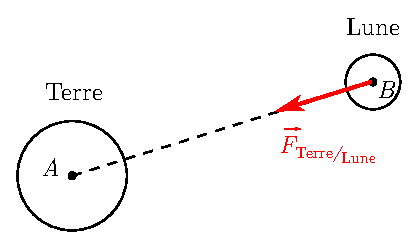
\includegraphics[width=.4\linewidth]{force}
\end{center}

\vspace{1em}

\begin{aconnaitre}[\MotDefinition{Caractéristiques d'une force}{}]
Une force est caractérisée par :
\begin{itemize}
\item son \textbf{point d'application} (origine du vecteur, ici $B$) ;
\item sa \textbf{droite d'action} ou \emph{direction} (droite support du vecteur, ici $(AB)$) ;
\item son \textbf{sens} (ici de $B$ vers $A$) ;
\item sa \textbf{valeur} ou \textbf{intensité} (c'est la \emph{norme} du vecteur, ici $\norme{\vect{F}_\text{Terre/Lune}}$), dont l'unité est le newton (symbole : N).

Attention, en physique la norme d'un vecteur est notée tout simplement en enlevant la flèche : $\norme{\vect{F}_\text{Terre/Lune}}$ est notée $F_\text{Terre/Lune}$.
\end{itemize}
\end{aconnaitre}

\vspace{1em}


Le \textbf{\MotDefinition{newton}{}} (symbole : N) équivaut à 1\unittrois{kg}{m}{s}{-2} : cela signifie qu'un Newton est la force colinéaire au mouvement qui, appliquée pendant une seconde à un objet d'un kilogramme, est capable d'ajouter (ou de retrancher) un mètre par seconde à sa vitesse.

\vspace{1em}


Cette petite pomme de 100\,g (figure ci-dessous) applique sur la table où elle est posée une force de 1\,N environ (attention, toutes les forces s'appliquant sur la pomme ne sont pas représentées sur cette figure). La force est représentée ci-dessous à l'échelle.

\begin{center}
    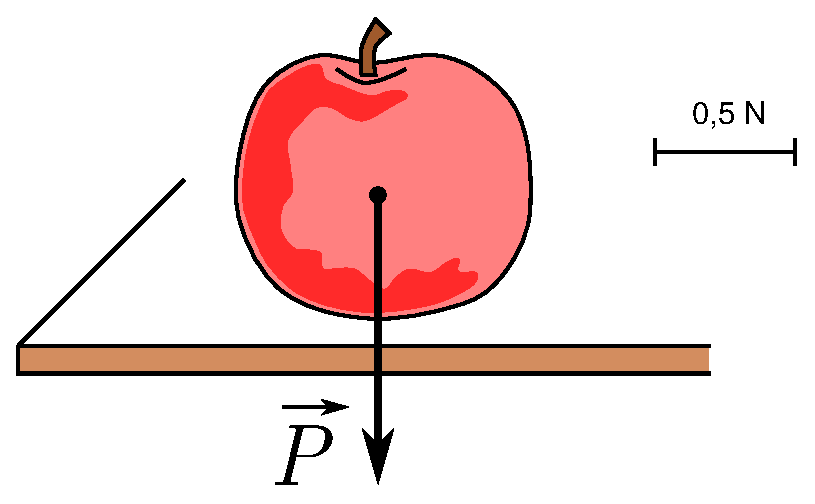
\includegraphics[width=.3\linewidth]{pomme}
\end{center}

\vspace{1em}

L'appareil qui mesure l'intensité de la force est le \textbf{\MotDefinition{dynamomètre}{}}. Il est constitué d'un ressort qui se déforme sous l'action de la force exercée. Un curseur indique alors l'intensité de la force à laquelle le dynamomètre est soumis. Figures ci-dessous : à gauche, différents dynamomètres linéaires et à droite, un dynamomètre circulaire.


\begin{center}
    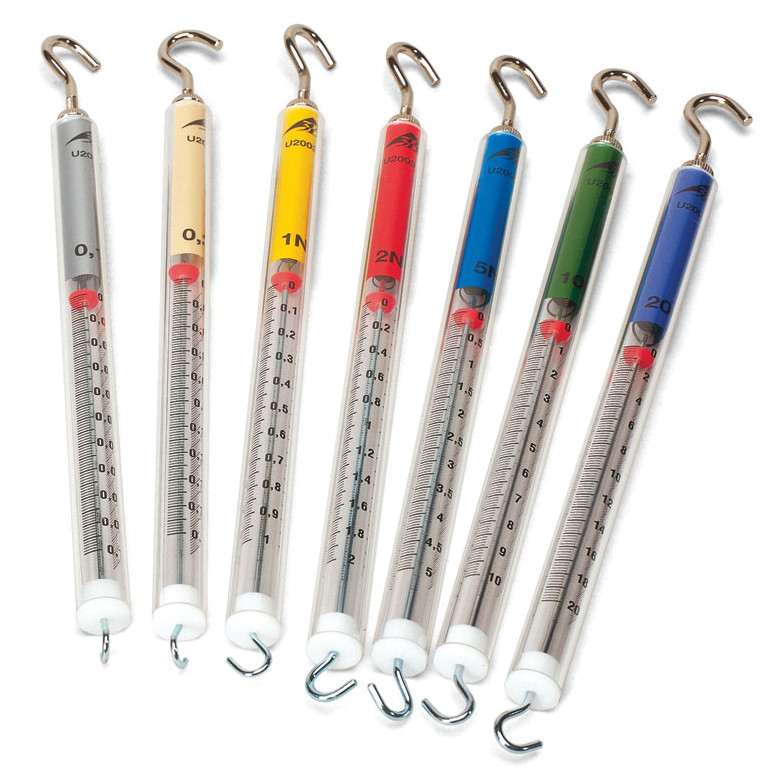
\includegraphics[width=.3\linewidth]{dynamometre}%
    \hfill%
    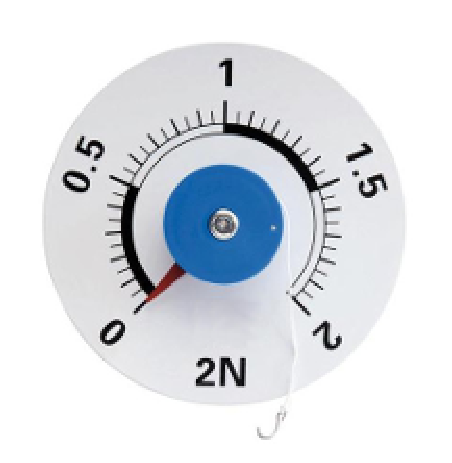
\includegraphics[width=.3\linewidth]{dynamometreRond}
\end{center}



\section{Force et vecteur}\label{ForceVecteur}

\subsection{Rappels sur les vecteurs}

Considérons le vecteur $\vect{AB}$ ci-dessous.

\begin{center}
    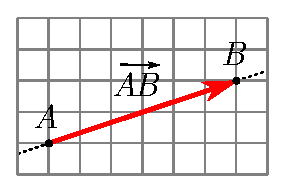
\includegraphics[width=.3\linewidth]{vecteurAB}
\end{center}

\vspace{1em}

Le \MotDefinition{vecteur}{} est un objet mathématique qui contient beaucoup d'informations : une \emph{droite d'action} (\emph{direction} en mathématiques), donnée par la droite passant par le vecteur, dite droite support (ici $(AB)$) ; un \emph{sens}, le long de la droite support (ici de $A$ vers $B$) ; une \emph{intensité} en newton (\emph{norme} en mathématiques), représentée par la taille du vecteur et notée $\norme{\vect{AB}}$.

C'est cet objet qui est utilisé pour représenter les forces en physique, car il contient toutes les informations permettant de les décrire. Le tableau ci-dessous donne la correspondance entre les noms utilisés en physique pour les forces et les propriétés mathématiques du vecteur :

\begin{center}
\renewcommand*\tabularxcolumn[1]{>{\centering\arraybackslash}m{#1}}
\begin{Ltableau}{.8\linewidth}{4}{c}
\hline
\multicolumn{2}{|c|}{\textbf{Vecteur en mathématiques}} & \multicolumn{2}{c|}{\textbf{Force en physique}} \\ \hline
\emph{Nom} & \emph{Notation}& \emph{Nom} & \emph{Notation} \\ \hline
direction & $(AB)$ & \MotDefinition{droite d'action}{} & $(AB)$ \\ \hline
sens & de $A$ vers $B$ & \MotDefinition{sens}{} & de $A$ vers $B$ \\ \hline
norme & $\norme{\vect{AB}}$ & \MotDefinition{intensité}{} (en N) & $AB$\\ \hline
\phantom{point d'application} & & \MotDefinition{point d'application}{} & $A$ \\ \hline
\end{Ltableau}
\end{center}


\begin{methode}[Représenter une force à l'aide d'un vecteur \MethodeRefExercice{representeVecteur}]
\label{methodeForceEchelle}
Pour représenter une force $\vect{T}$ d'intensité 600\,N à l'aide d'un vecteur, il faut choisir une échelle adaptée, par exemple 1\,cm représente 150\,N, puis tracer sur la droite d'action un vecteur de longueur 4\,cm (car $4\times 150=600$) à partir du point d'application.

L'échelle choisie ne doit être ni trop petite ni trop grande. Elle doit permettre au vecteur d'utiliser au mieux l'espace disponible sur la feuille.

\exercice
Représenter la force $\vect{F}$ dont l'intensité est de 625\,N, la droite d'action (MN), le sens de N à M et le point d'application $G$.

\correction
\vspace{.5em}
\begin{tikzpicture}[general]
\draw[quadrillage55] (0,0) grid (7,3);
\pointGraphique{2}{.5}{M}{below left};
\pointGraphique{6}{2.5}{N}{below right};
\pointGraphique{5}{2}{G}{below right};
\end{tikzpicture}
\end{methode}




\subsection{Addition de vecteurs}

Pour additionner deux vecteurs $\vect{u}$ et $\vect{v}$, deux méthodes peuvent être utilisées. Le vecteur somme $\vect{u+v}$ alors obtenu est le même dans les deux cas. 

Considérons les deux vecteurs $\vect{u}$ et $\vect{v}$ ci-dessous.

\begin{center}
    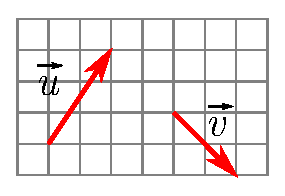
\includegraphics[width=.3\linewidth]{vecteurSomme1}
\end{center}


\begin{methode}[Addition de vecteurs : méthode \og bout à bout \fg \MethodeRefExercice{exAddVect}]
\label{methodeAddBoutBout}

Pour additionner les deux vecteurs $\vect{u}$ et $\vect{v}$, on les place l'un au bout de l'autre. Le vecteur somme $\vect{u+v}$ a pour origine le début du premier vecteur et pour fin l'endroit où se termine le second.

\begin{center}
    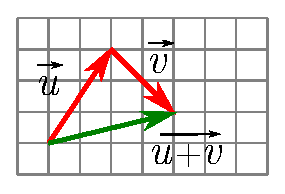
\includegraphics[width=.4\linewidth]{vecteurSomme2}
\end{center}

\exercice
En utilisant la méthode bout à bout, faire la somme des vecteurs $\vect{F}$ et $\vect{T}$.

\correction
\vspace{.5em}
\begin{tikzpicture}[general]
\draw[quadrillage55] (0,0) grid (7,3);
\draw[axe] (1,1)--(2,2.5);
\draw[axe] (4,2.5)--(6,1.5);
\draw (1.2,1.7) node[above] {$\vect{F}$};
\draw (5,2) node[above] {$\vect{T}$};
\end{tikzpicture}
\end{methode}


\begin{methode}[Addition de vecteurs : méthode du parallélogramme \MethodeRefExercice{exAddVect}]
\label{methodeAddParall}

Pour additionner les deux vecteurs $\vect{u}$ et $\vect{v}$, on les place de telle sorte qu'ils aient même origine et on trace le parallélogramme ainsi défini (en pointillés sur la figure ci-dessous). La diagonale du parallélogramme correspond au vecteur somme $\vect{u+v}$.

\begin{center}
    \includegraphics[width=.4\linewidth]{vecteurSomme3}
\end{center}

\exercice
En utilisant la méthode du parallélogramme, faire la somme des vecteurs $\vect{F}$ et $\vect{T}$.
\correction
\vspace{.5em}
\begin{tikzpicture}[general]
\draw[quadrillage55] (0,0) grid (7,3);
\draw[axe] (1,1)--(2,2.5);
\draw[axe] (4,2.5)--(6,1.5);
\draw (1.2,1.7) node[above] {$\vect{F}$};
\draw (5,2) node[above] {$\vect{T}$};
\end{tikzpicture}
\end{methode}



\vspace{2em}

\begin{remarque}
Attention ! Notons bien que $\norme{\vect{u} + \vect{v}} \neq \norme{\vect{u}} + \norme{\vect{v}}$, ce qui est particulièrement trompeur en physique où on écrit $u$ la valeur (norme) du vecteur $\vect{u}$, ce qui donne $(u+v) \neq u + v$... 

C'est ce que montre l'exemple ci-dessous. Les vecteurs $\vect{u}$ et $\vect{v}$ ont pour intensité 2\,N. Le vecteur somme $\vect{u+v}$ a pour intensité 2,8\,N.
\begin{center}
    \begin{tikzpicture}[general]
    \draw[quadrillage55] (0,0) grid (8,3);
    \draw[axe] (1,.5)--(1,2.5); \draw (.5,1.5) node {$\vect{u}$};
    \draw[axe] (2,.5)--(4,.5); \draw (3,1) node {$\vect{v}$};
    \draw[axe] (5,.5)--(7,2.5); \draw (6.5,1) node[above] {$\vect{u+v}$};
    \draw (6,-.25) node {échelle : 2 carreaux $\rightarrow$ 1\,N};
\end{tikzpicture}
\end{center}

\end{remarque}







\section{Résultante des forces}

\begin{aconnaitre}[Résultante d'une force]
Lorsque plusieurs forces sont appliquées sur un même objet, on peut calculer la \textbf{\MotDefinition{résultante des forces}{}}, qui est l'\textbf{addition vectorielle de toutes les forces appliquées} sur l'objet.

\vspace{1em}

\textbf{Tout se passe alors comme si l'objet n'était soumis qu'à la résultante des forces.}


\begin{center}
    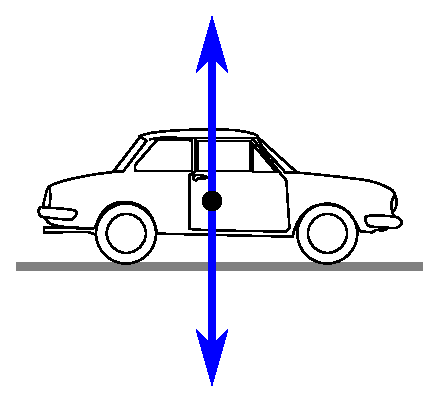
\includegraphics[width=.25\linewidth]{resultante1}%
    \hfill%
    \includegraphics[width=.55\linewidth]{resultante2}
\end{center}

{\footnotesize Figure de gauche, la résultante des forces est nulle : tout se passe comme si la voiture n'était soumise à aucune force. Figure de droite, la résultante des forces est non nulle : tout se passe comme si la voiture était soumise à une force dirigée vers la droite : la \emph{force résultante}.}

\end{aconnaitre}












\section{Corde et poulie}


Lorsqu'on applique une force à l'extrémité d'une \textbf{\MotDefinition{corde}{}}, la droite d'action de la force est toujours située le long de la corde. La corde transmet intégralement la force : si on tire avec une force d'intensité 1\,N à l'extrémité de la corde, le dynamomètre va indiquer 1\,N (voir figures ci-dessous).


Une \textbf{\MotDefinition{poulie}{}} ne modifie pas l'intensité d'une force, mais elle permet d'orienter différemment sa droite d'action (voir ci-dessous).

\vspace{1em}

\begin{center}
    \includegraphics[width=.7\linewidth]{cordePoulie}
\end{center}

\vspace{2em}

\begin{remarque}
notez bien que la force est nommée $\vect{F}$ (grandeur vectorielle), mais que l'intensité de la force est nommée $F$ (grandeur scalaire correspondant à $\norme{\vect{F}}$).
\end{remarque}





\section{Principe des actions réciproques}

Comme montré sur la figure ci-dessous, lorsque le skater pousse le mur avec sa main, alors le mur exerce sur lui une force égale en intensité mais de sens opposé. C'est ce qui permet au skater de se mettre en mouvement vers la droite dans ce cas.

\begin{center}
    \includegraphics[width=.4\linewidth]{skater}
\end{center}

% il faut ajouter la force du mur sur le skater
% de plus il faut modéliser la situation à côté

Si on étudie le système \{skater\}, il subit de la part du mur la force $\vect{F}_\text{mur/skater}$. La force que le skater applique sur le mur n'est pas une force subie par le système, donc ne nous intéresse pas dans ce cas. 

\vspace{1em}

\begin{aconnaitre}[Principe des \MotDefinition{actions réciproques}{} (3\up{e} loi de Newton)]

Lorsqu'un objet $A$ exerce sur un objet $B$ une force $\vect{F}_{A/B}$, alors l'objet $B$ exerce sur l'objet $A$ une force $\vect{F}_{B/A}$ telle que : {\large\[\vect{F}_{A/B} = -\vect{F}_{B/A}\]}

\begin{center}
    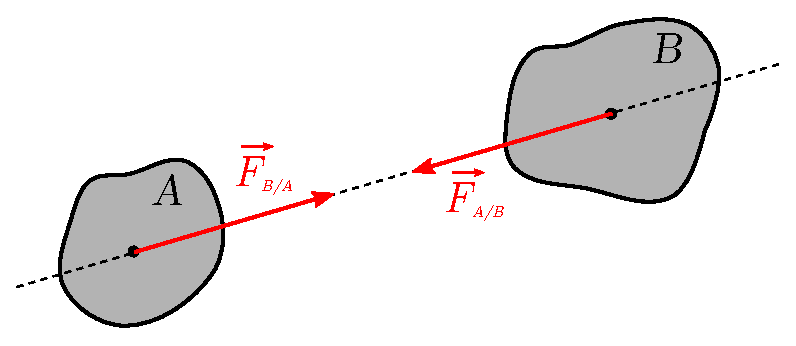
\includegraphics[width=.5\linewidth]{3eLoi}
\end{center}
\end{aconnaitre}
  


\begin{remarque}
lorsqu'un objet applique sur un autre objet une action mécanique, alors celui-ci applique en retour une action mécanique égale mais opposée. Une action mécanique n'existe donc jamais seule et c'est la raison pour laquelle on dit qu'il existe entre deux objets une \textbf{\MotDefinition{interaction}{}} : l'action du premier induit une action en retour du second. 
\end{remarque}


La \textbf{propulsion} repose sur le principe des actions réciproques : comme pour le skater on \og pousse \fg le sol vers l'arrière avec nos pieds afin d'être propulsé vers l'avant : c'est l'action réciproque qui s'exerce sur le système qui le propulse vers l'avant. Et si le sol est verglacé, alors on n'arrive pas à le \og pousser \fg (pas de frottement) et du coup on n'est pas propulsé vers l'avant.

Autres exemples de propulsion : les rames poussent l'eau en arrière pour faire avancer le bateau ; les roues \og pousse \fg la route vers l'arrière afin de faire avancer la voiture ; l'oiseau \og pousse \fg l'air avec ses ailes pour avancer.





\section{Diagramme objets--interactions et modélisation}

Le \MotDefinition{diagramme objets--interactions}{} (DOI) permet de modéliser facilement une situation. Il dresse l'inventaire de tous les objets en interaction avec le système. À chaque interaction mentionnée correspond une force dans la modélisation.

\begin{methode}[Construction d'un diagramme objets--interactions\MethodeRefExercice{doiFirst}]
\label{methodeDOI}

Pour construire un diagramme objets--interactions, il faut :
\begin{enumerate}
\item placer l'objet étudié (le système) dans un rectangle entouré par des traitillés 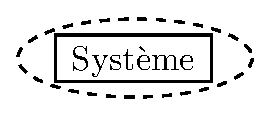
\includegraphics[width=2cm]{DOIsysteme};
\item énumérer tous les objets en interaction avec le système et les représenter dans des rectangles 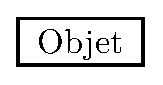
\includegraphics[width=1.2cm]{DOIobjet} ; 
\item représenter par des flèches en trait plein et à deux pointes (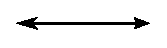
\includegraphics[width=1cm]{DOIflecheP}) les interactions de contact entre les objets et le système ;
\item représenter par des flèches en traitillé et à deux pointes (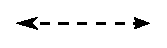
\includegraphics[width=1cm]{DOIflecheT}) les interactions à distance entre les objets et le système ;
\item auprès de chaque flèche, décrire l'interaction ;
\item ne pas oublier la légende.
\end{enumerate}


\vspace{1em}

Exemple : dans la situation à gauche ci-dessous, on étudie la voiture (arrêtée). À droite, le diagramme objets--interactions correspondant.


\begin{center}
    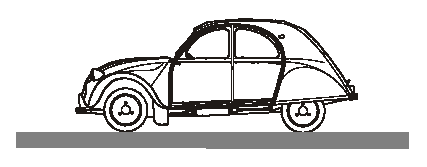
\includegraphics[width=.4\linewidth]{voiture}%
    \hfill%
    \includegraphics[width=.5\linewidth]{DOIexemple}
\end{center}

\exercice
Construire le diagramme objets-interactions pour un grêlon tombant du ciel (système étudié : le grêlon).
\correction
\vspace{4cm}
\phantom{.}
\end{methode}


\begin{remarque}
lorsque la vitesse d'un objet est faible et/ou que sa masse volumique est largement plus grande que celle de l'air, on néglige l'action de l'air sur le système. C'est le cas dans l'exemple ci-dessus.
\end{remarque}

\vspace{1em}

\begin{aconnaitre}[Du DOI aux forces appliquées au système]
La modélisation d'une situation à partir d'un diagramme objets--interactions est aisée : à chaque interaction mentionnée dans le diagramme objets--interactions correspond une force appliquée au système étudié.
\end{aconnaitre}

\vspace{1em}

Pour l'exemple de la voiture, il y a deux interactions dans le DOI donc le système \{voiture\} est soumis à deux forces appelées ici $\vect{P}$ (le poids) et $\vect{R}$ (la réaction du support) :

\begin{center}
    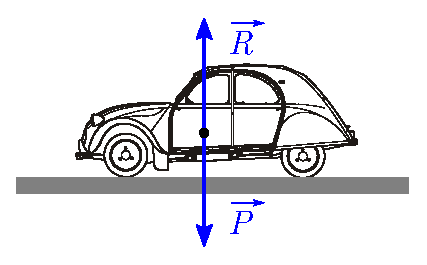
\includegraphics[width=.4\linewidth]{voitureForce}%
    \hfill%
    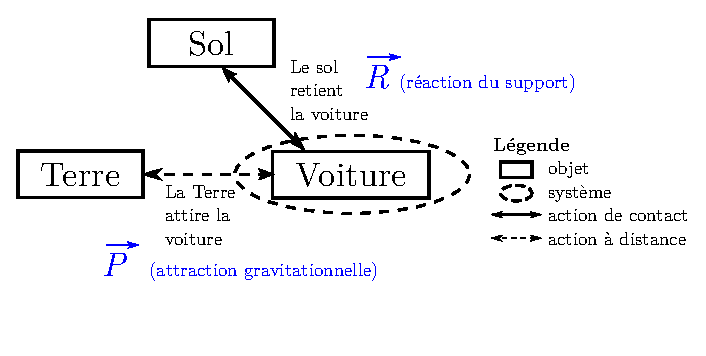
\includegraphics[width=.4\linewidth]{DOIexempleForce}
\end{center}



\begin{aconnaitre}[Le cas de l'air dans les DOI]
La force exercée par l'air sur le système étudé est négligeable devant les autres forces dans deux cas :
\begin{itemize}
    \item le système possède une vitesse nulle ou faible ;
    \item la masse volumique du système est très grande devant celle de l'air.
\end{itemize}

\vspace{.5em}
Ainsi, on peut négliger l'action de l'air pour une voiture arrêtée ou roulant à faible vitesse, mais pas pour une montgolfière qui <<\,flotte\,>> dans les airs.  
\end{aconnaitre}





\section{Les différentes forces que l'on va rencontrer}

\begin{minipage}[c]{.65\linewidth}
Le \textbf{\MotDefinition{poids}{}} est toujours présent lorsqu'un objet se trouve sur Terre, il est dû à l'attraction gravitationnelle exercée par la Terre sur l'objet. Ci-contre, un objet en chute libre proche de la surface de la Terre. L'objet n'est soumis qu'à son poids $\vect{P}$. Le poids a toujours pour droite d'action la verticale et pour sens vers le bas.
\end{minipage}\hfill%
\begin{minipage}[c]{.33\linewidth}
\begin{center}
    \includegraphics[width=.25\linewidth]{ForcePoids}
\end{center}
\end{minipage}

\vspace{2em}

\begin{minipage}[c]{.65\linewidth}
Lorsqu'un objet est posé sur un support, il subit de la part de ce dernier une force de réaction qui s'oppose à son poids (selon le principe des actions réciproques). Ci-contre, un objet posé sur le sol. L'objet est soumis à son poids $\vect{P}$ et à la \textbf{\MotDefinition{réaction du support}{}} $\vect{R}$ qui l'empêche de s'enfoncer dans le support. La réaction du support a toujours pour droite d'action la perpendiculaire au support et pour sens du support vers le haut.
\end{minipage}\hfill%
\begin{minipage}[c]{.33\linewidth}
\begin{center}
    \includegraphics[width=.6\linewidth]{ForceReactionSupport1}
\end{center}
\end{minipage}

\vspace{2em}

\begin{minipage}[c]{.65\linewidth}
Si le support est un plan incliné, deux forces s'appliquent à l'objet : la réaction du support $\vect{R}$ qui empêche l'objet de s'enfoncer dans le support et une \textbf{\MotDefinition{force de frottement}{}} $\vect{f}$ qui empêche l'objet de glisser. La force de frottement a pour droite d'action la parallèle au support et pour sens l'opposé de celui du mouvement (ou du mouvement potentiel) de l'objet.

Notons que si l'objet ne bouge pas (équilibre) $\vect{R_N} + \vect{f} = -\vect{P}$.

\vspace{2em}

\end{minipage}\hfill%
\begin{minipage}[c]{.33\linewidth}
\begin{center}
    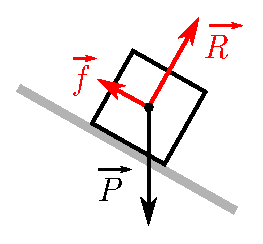
\includegraphics[width=.55\linewidth]{ForceReactionSupport3}
\end{center}
\end{minipage}




\begin{minipage}[c]{.65\linewidth}
Lorsqu'un objet est suspendu à un fil, une \MotDefinition{force de tension}{} $\vect{T}$ apparaît : c'est la force qui retient l'objet et lui évite la chute. La force de tension est toujours dans la même direction que le fil.
\end{minipage}\hfill%
\begin{minipage}[c]{.33\linewidth}
\begin{center}
    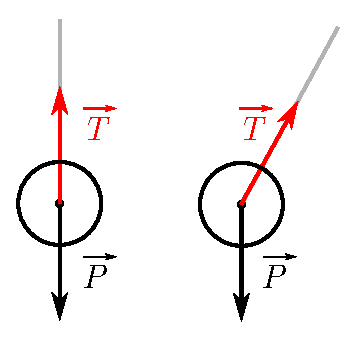
\includegraphics[width=.8\linewidth]{ForceTensionFil}
\end{center}
\end{minipage}


Les paragraphes suivants listent les différentes forces rencontrées cette année.

\vspace{1em}

Lorsqu'un objet subit une traction (par exemple par un moteur ou parce qu'on le tire), on parle de \MotDefinition{force de traction}{} ;

\vspace{1em}

Lorsqu'un objet est propulsé (par exemple par un moteur ou encore parce qu'on le pousse), on parle de \MotDefinition{force de propulsion}{} ;

\vspace{1em}

Lorsqu'un objet avance avec une grande vitesse dans l'air ou dans un fluide, des frottements apparaissent : cette \MotDefinition{force de frottement}{} est toujours orientée dans le sens opposé à celui du mouvement et sa droite d'action est celle du déplacement de l'objet ; 

\vspace{1em}

Deux charges électriques de signes opposés s'attirent, de même signe se repoussent : on parle de \MotDefinition{force électrique}{} ;

\vspace{1em}

Un aimant attire les matériaux ferreux : on parle de \MotDefinition{force magnétique}{} ;

\vspace{1em}

Un objet plongé dans un fluide subit une force verticale dirigée vers le haut : la \MotDefinition{poussée d'Archimède}{} (se reporter au chapitre sur pression et hydrostatique).










